\documentclass[border=6pt]{standalone}
\usepackage[T1]{fontenc}
\usepackage{courier}
\usepackage[scaled=0.95]{helvet}
\renewcommand{\familydefault}{\sfdefault}
\usepackage{sfmath}
\usepackage[version=4]{mhchem}
\usepackage{tikz}
\usepackage{pgfplots}
\pgfplotsset{compat=newest}
\usetikzlibrary{arrows.meta,positioning,calc,fit,backgrounds,shapes.geometric,decorations.pathreplacing,patterns}
\definecolor{ink}{HTML}{17233A}
\definecolor{inksoft}{HTML}{44506A}
\definecolor{teal}{HTML}{0E6B6B}
\definecolor{tealsoft}{HTML}{E5F0EF}
\definecolor{amber}{HTML}{B26B12}
\definecolor{ambersoft}{HTML}{FBF0DF}
\definecolor{blue}{HTML}{2F6690}
\definecolor{bluesoft}{HTML}{E3ECF4}
\definecolor{plum}{HTML}{7A4D8C}
\definecolor{plumsoft}{HTML}{EFE7F3}
\definecolor{greyc}{HTML}{8A94A3}
\definecolor{linec}{HTML}{D3DCE1}
\definecolor{oxy}{HTML}{C0392B}
\definecolor{carb}{HTML}{3B4252}
\definecolor{hyd}{HTML}{E6E9EE}
\definecolor{nit}{HTML}{2F6690}
\tikzset{
  every picture/.style={line cap=round,line join=round},
  lab/.style={font=\small, text=inksoft},
  >={Stealth[length=7pt]},
}
\pgfplotsset{
  every axis/.append style={axis line style={inksoft}, tick style={inksoft}, tick label style={font=\footnotesize, text=inksoft}, label style={font=\small, text=ink}},
}
% fragment tile: \frag{node name}{position}{colour}{content}
\newcommand{\frag}[4]{\node[draw=#3, fill=#3!12, line width=1.4pt, rounded corners=6pt, minimum width=1.25cm, minimum height=1.05cm, text=#3, font=\bfseries] (#1) at (#2) {#4};}
\newcommand{\ring}{\tikz[baseline=-0.6ex]{\draw[line width=1.1pt] (0:0.3)--(60:0.3)--(120:0.3)--(180:0.3)--(240:0.3)--(300:0.3)--cycle; \draw[line width=0.8pt] (0,0) circle (0.16);}}
\newcommand{\bond}[2]{\draw[ink, line width=2.2pt] (#1) -- (#2);}

\begin{document}
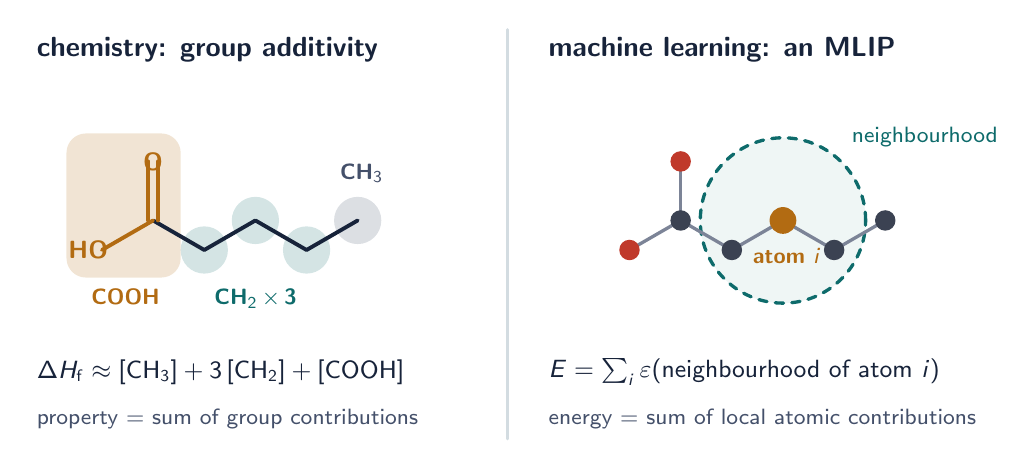
\begin{tikzpicture}
\node[font=\bfseries, text=ink, anchor=west] at (-0.2,2.55) {chemistry: group additivity};
\fill[amber, fill opacity=0.18, rounded corners=7pt] (0.30,-0.35) rectangle (1.75,1.48);
\fill[teal, fill opacity=0.18] (2.050,0.000) circle (0.3);
\fill[teal, fill opacity=0.18] (2.699,0.375) circle (0.3);
\fill[teal, fill opacity=0.18] (3.349,0.000) circle (0.3);
\fill[greyc, fill opacity=0.3] (3.998,0.375) circle (0.3);
\draw[ink, line width=1.4pt] (1.400,0.375) -- (2.050,0.000);
\draw[ink, line width=1.4pt] (2.050,0.000) -- (2.699,0.375);
\draw[ink, line width=1.4pt] (2.699,0.375) -- (3.349,0.000);
\draw[ink, line width=1.4pt] (3.349,0.000) -- (3.998,0.375);
\draw[amber, line width=1.4pt] (1.340,0.375) -- (1.340,1.125);\draw[amber, line width=1.4pt] (1.460,0.375) -- (1.460,1.125);
\draw[amber, line width=1.4pt] (1.400,0.375) -- (0.750,0.000);
\node[font=\small\bfseries, text=amber, fill=white, fill opacity=0, text opacity=1, inner sep=1pt] at (1.400,1.125) {O};
\node[font=\small\bfseries, text=amber, inner sep=1pt, anchor=east] at (0.870,0.000) {HO};
\node[font=\footnotesize\bfseries, text=amber] at (1.05,-0.60) {COOH};
\node[font=\footnotesize\bfseries, text=teal] at (2.70,-0.62) {CH$_2$\,$\times$\,3};
\node[font=\footnotesize\bfseries, text=inksoft] at (4.05,0.97) {CH$_3$};
\node[font=\small, text=ink, anchor=west] at (-0.2,-1.55) {$\Delta H_\mathrm{f} \approx [\mathrm{CH_3}] + 3\,[\mathrm{CH_2}] + [\mathrm{COOH}]$};
\node[font=\footnotesize, text=inksoft, anchor=west] at (-0.2,-2.15) {property = sum of group contributions};
\draw[linec, line width=1pt] (5.9,-2.4) -- (5.9,2.8);
\node[font=\bfseries, text=ink, anchor=west] at (6.3,2.55) {machine learning: an MLIP};
\draw[teal, dashed, line width=1.2pt, fill=tealsoft, fill opacity=0.6] (9.399,0.375) circle (1.05);
\draw[inksoft!70, line width=1.2pt] (8.100,0.375) -- (8.750,0.000);
\draw[inksoft!70, line width=1.2pt] (8.750,0.000) -- (9.399,0.375);
\draw[inksoft!70, line width=1.2pt] (9.399,0.375) -- (10.049,0.000);
\draw[inksoft!70, line width=1.2pt] (10.049,0.000) -- (10.698,0.375);
\draw[inksoft!70, line width=1.2pt] (8.100,0.375) -- (8.100,1.125);
\draw[inksoft!70, line width=1.2pt] (8.100,0.375) -- (7.450,0.000);
\fill[carb] (8.100,0.375) circle (0.13);
\fill[carb] (8.750,0.000) circle (0.13);
\fill[carb] (9.399,0.375) circle (0.13);
\fill[carb] (10.049,0.000) circle (0.13);
\fill[carb] (10.698,0.375) circle (0.13);
\fill[oxy] (8.100,1.125) circle (0.13);
\fill[oxy] (7.450,0.000) circle (0.13);
\fill[amber] (9.399,0.375) circle (0.17);
\node[font=\footnotesize\bfseries, text=amber] at (9.45,-0.08) {atom $i$};
\node[font=\footnotesize, text=teal, anchor=west] at (10.15,1.43) {neighbourhood};
\node[font=\small, text=ink, anchor=west] at (6.3,-1.55) {$E = \sum_i \varepsilon(\text{neighbourhood of atom } i)$};
\node[font=\footnotesize, text=inksoft, anchor=west] at (6.3,-2.15) {energy = sum of local atomic contributions};
\end{tikzpicture}
\end{document}
